\documentclass[11pt]{article}
\usepackage[utf8]{inputenc}
\usepackage{amsmath}
\DeclareMathOperator*{\argmin}{arg\,min}
\usepackage{setspace}
\usepackage{threeparttable}
\usepackage{graphicx}
\usepackage{subcaption}
\usepackage{geometry}
\usepackage[backend=biber,style=authoryear,sorting=ynt]{biblatex}
\addbibresource{mlbibliography.bib}
\geometry{margin=1in}
\graphicspath{ {images/} }
\usepackage{wrapfig}
\renewcommand{\topfraction}{0.85}
\renewcommand{\bottomfraction}{0.85}

\title{Estimating Idiosyncratic Price Setting Behavior with Machine Learning}
\author{Michael Munsell \footnote{Department of Economics, Brandeis University, mmunsell@brandeis.edu}}
\date{October 2018}

\begin{document}


\maketitle

%Line spacing
\onehalfspacing
\setlength{\parindent}{2em}

\begin{abstract}
When price  setting  behavior  is  assumed  to  be  endogenous, as  in  state-dependent pricing models,  the  firms  that  change  prices  are  those  that  are  furthest  away  from  their  optimal desired  price. A substantial hurdle in empirically identifying state-dependent pricing behavior lies in the difficulty of estimating a firm's desired price ($p^*$), which is unobservable to the econometrician. In this paper, we provide intuition on how a standard idiosyncratic price setting model can be mapped to various machine learning methods, and then empirically test the ability of these methods to predict out-of-sample good-level price setting behavior. Using a subset of online grocery price data, we demonstrate that machine learning methods show modest improvements over traditional econometric approaches in estimating the direction of price changes as well as the magnitude of adjustment. To determine whether these modest gains have an applied value, we demonstrate that the best performing machine learning algorithm ($k$-nearest neighbor) is able to anticipate good-level price increases at a rate twice that of a traditional linear model. In line with state-dependent price theory, the algorithm with the ability to better anticipate good-level inflation also estimated a relatively larger deviation between the good's estimated desired price and its current price.
\end{abstract}

%Keywords: Machine learning, State-dependent pricing, Online data   


\vspace{4cm}


\pagebreak{}
\doublespacing


\section{Introduction}
Over the past two decades, the growing availability of micro price data has led to a wealth of studies that evaluate the impact of firm-level pricing behavior on business cycle dynamics. This ability to explore the fundamental economic forces that drive aggregate inflation has had a significant impact on macroeconomic modeling. In the seminal paper by Bils and Klenow (2004), the authors found much more violate inflation among sticky-priced goods using disaggregate CPI data than what was generally predicted by the macro models of the time. Furthermore, price setting behavior differed markedly across product type, reinforcing the need for heterogeneity in models that may have previously relied on a representative agent approach. A thorough review by Klenow and Malin (2010) provides a more complete description of this body of literature and its subsequent impact. 

The ability to evaluate firm-level pricing decisions through micro data allows the economist to further understand the endogenous process of price setting, which can be reflected most directly in the theory of state-dependent pricing. When price  setting  behavior  is  assumed  to  be  endogenous, as is the case  in  state-dependent pricing models,  the  firms  that  change  prices  are  those  that  are  furthest  away  from  their  optimal  frictionless  price  (the  price  the  firm  would  select  if  it  could  adjust  its  price  with  no  cost),  a  mechanism  coined  by  Golosov  and  Lucas  (2007) as  the  selection  effect. This can be contrasted with time-dependent pricing, where a firm is only allowed to change its price at a random, exogenously determined time period.  During  times  of  monetary  expansion,  firms  that  adjust  prices  in state-dependent models will  be  those  that  require  the  largest  price  change,  which  adds  a  greater  degree  of  flexibility  to  the  aggregate  price  level  and  dampens  the  impact  of  any  intervention  on  real  economic  output. 

It is difficult to identify state-dependent pricing using actual data for many reasons, however, a primary and substantial hurdle is the fact that state-dependent pricing relies on the estimation of a firm's desired price ($p^*$), which is unobservable. Therefore, many papers that attempt to establish a measure of $p^*$ rely on indirect methods of identification (e.g., Carvalho and Kryvtsov (2018), Bils, Klenow and Malin (2012)) or calibrate models to better reflect key features of the micro data (e.g., Burstein and Hellwig (2007), Kryvtsov and Midrigan (2012)). Therefore, in this paper we are motivated by the ability to estimate a measure of $p^*$ \textit{directly}. Specifically, we compare the ability of a standard econometric model to accurately predict out-of-sample price setting behavior to that of methods borrowed from the machine learning literature. Due to the empirical benefits of estimating a firm's optimal desired price, determining the method that exhibits the greatest ability to anticipate price setting behavior will have direct implications for measuring the effectiveness of macroeconomic interventions.  


The last several years have seen an explosion of studies that attempt to use machine learning methods to predict various economic phenomenon, such as consumer demand and behavior (Peysakhovich and Naecker
(2017), Bajari, Nekipelov, Ryan, and Yang (2015)) and even optimal model selection (Duarte (2018)). This rise in the use of machine learning within the discipline of economics has been met with a healthy dose of skepticism, and the authors of this paper acknowledge that this can be for good reason. In a 2017 review, Mullainathan and Spiess effectively establish a practical guide for the responsible use of machine learning in applied econometrics. Given that the objective function for most machine learning algorithms are designed to minimize out of sample prediction error, their insights are most directly aligned with applications where improved predicted outcomes have applied value, and \textit{not} applications that require direct parameter estimation and/or interpretation. Given that predicted $p^*$, when estimated as accurately as possible, provides a measure of how far a firm currently is from its ideal price, we believe that idiosyncratic price setting behavior is well suited for the machine learning toolkit.   

Using a publicly available micro price dataset of U.S. online grocery items, we estimate two primary price setting behaviors across a subsample of known price change observations; 1) the decision to increase vs. decrease a price, and 2) the magnitude of the price change, conditional on adjustment. We first employ a standard logistic and linear model rooted in state-dependent price theory. These models, as standard with the current literature, incorporate the aggregate price level in the economy as an explanatory variable. Next, we move to machine learning methods that expands the right hand side of the econometric model by disassembling the aggregate price level into individual competitor's prices, unique for each good-level observation. One key benefit of machine learning methods are their ability to handle high dimensional data that is typically not supported by the regression framework. Our logic for relying on individual competitor's prices rather than the aggregate price level assumes that firms are more impacted by their competitors' price directly than the general price level in the economy. We begin with a linear machine learning model (Ridge) for a more direct comparison to that of the standard econometric approach, and then move to the non-linear approaches of random forest and $k$-nearest neighbors, which have continually demonstrated superior out-of-sample prediction in many machine learning applications. 

Results show that out-of-sample prediction of price setting behavior is improved using machine learning methods and dissaggregated competitor price data compared with traditional econometric approaches. Gains are more substantial when predicting price change direction (i.e., price increase or decrease) than good-level inflation rates, and a non-linear framework appears to increase the gains in out-of-sample prediction even further. However, particularly in the case of predicting the magnitude of a price change, these gains in out-of-sample prediction are modest and demonstrate the known difficulty of estimating idiosyncratic price setting behavior using only micro price data.

To see if these modest gains have any empirical impact, we complete an exercise similar to that of Bils, Klenow and Malin's (2012) concept of reset inflation. This exercise is the most direct application of an estimated optimal price $p^*$ in that a firm's estimated optimal inflation rate is applied to its current price during periods in which a price change does not occur. In essence, this exercise estimates the optimal price path for each good and the deviation of that optimal price from the good's current price. While Bils, Klenow and Malin assume time-dependent pricing to estimate their $p^*$, we compare our baseline linear state-dependent estimation of $p^*$ to that of our best performing machine learning method. The $k$-nearest neighbor algorithm, which breaks the furthest from any defined economic model structure and represents a primarily data-driven estimation approach, accurately anticipates price increases in the data at a rate nearly double that of the linear method. In addition, prior to a realized price change (both increase and decrease), the $k$-nearest neighbor algorithm estimates a larger deviation in desired price from a firm's current price; a behavior that mimics state-dependent price theory. Further investigation is required to determine if this improvement in anticipating price setting behavior has a tangible impact on measuring the deviation of desired prices from the current price level in the aggregate economy.  

The remainder of the paper is structured as follows. Section 2 provides the underlying theoretical framework that informs our econometric model. Section 3 provides a description of the selected prediction methods, including the properties of each machine learning approach. Section 4 discusses our data source and further explains our approach for empirical estimation. Section 5 provides detailed results for the prediction exercise. Section 6 outlines the results of our reset inflation exercise, including robustness tests, and section 7 concludes.  
\section{Theoretical Framework}
\subsection{Model}

Our theoretical framework is in line with many standard state-dependent pricing models and largely follows the model outline in Bonomo, Silva Correa and Mederios (2018). For brevity, only the key components needed to understand our empirical applications are described below. Readers interested in the full model derivation can refer to the appendix of their working paper.  

We assume that there exists a continuum of monopolistically competitive firms that supply differentiated goods according to the following production function: 
%
$$Y_{i,t} = A_{i,t}L^{\alpha}_{i,t}M^{1-\alpha}_{t}$$
%
where $Y_{i,t}$ denotes an individual firm's final good, $A_{i,t}$ is the productivity factor, $L_{i,t}$ is labor, and $M_{t}$ represents a CES aggregate of intermediate goods (with $\alpha$ denoting the share of intermediate goods used in the production of the final consumption good). Following the work of Basu (1995) and Dotsey and King (2006), the model exhibits strategic complementarities through the presence of $\alpha$. Specifically, for values of $\alpha > 0$, each individual firm requires intermediate inputs from all other firms, generating a scenario where costs fully respond to a shock only if the price of other firms respond as well. While many consumption goods in online price datasets do not require intermediate inputs (e.g., grocery items, as used in this study), the concept of strategic complementarities represented in the model is highly relevant to online markets where the accessibility of competitors prices may easily influence the pricing decision of individual firms. 

In a frictionless environment (i.e., one in which a producer can continuously adjust prices), the perfectly flexible price for producer $i$ ($P^{*}_{i,t}$) is determined by a standard, profit maximizing markup rule:
%
\begin{equation} \label{eq:1} \frac{P^{*}_{i,t}}{P_{t}} = \mu \psi(Y_{i,t}, X_{t}, \xi_{t}, A_{i,t})
\end{equation}
%
where $\psi(.)$ is the real marginal cost function, $\mu$ is desired markup, $X_{t}$ is a vector of aggregate macroeconomic variables, and $\xi_{t}$ and $A_{i,t}$ are aggregate and idiosyncratic shocks, respectively. Log-linearization around the steady state equilibrium provides the firm's optimal price equation (lower case variables represents logarithms):

%
\begin{equation} \label{eq:2}
p^*_{i,t} = k + \theta x_{t} + (1-\theta)p_{t} + \widetilde\xi_{t} + \widetilde a_{i,t}
\end{equation}
%

with aggregate and idiosyncratic shocks approximated by
%
$$\widetilde\xi_{t} = \widetilde\xi_{t-1} + v_{t}, \quad  v_{t} 	\sim  \mathcal{N}(0,\sigma_{v}^{2})$$
$$\widetilde a_{i,t}  = \eta + \widetilde a_{i,t-1} + \epsilon_{i,t}, \quad \epsilon_{i,t} \sim  \mathcal{N}(0,\sigma^{2})$$
%
The variable $\theta$, which includes information contained in $\alpha$, helps to define the magnitude of strategic complementarities by determining the weight placed on competitors prices ($p_{t}$) relative to other aggregate variables in the macro economy.

\subsection{State-Dependent Pricing}
If we assume that firms follow an $Ss$ pricing policy, with state variable $r^{*}_{i,t} = p_{i,\tau} - p^{*}_{i,t}$ and $\tau$ representing the time of last price adjustment, we can postulate the optimal pricing policy of firm $i$, given that we cannot view the frictionless optimal price defined in equation (2). Standard with $Ss$ pricing, if $r^{*}_{i,t}$ reaches an upper bound $S$ (unknown to the econometrician), the firm's optimal price will be much lower than its current price and the firm will be willing to pay any menu cost associated with decreasing its price. Similarly, if $r^{*}_{i,t}$ reaches the lower bound $s$, the firm's optimal price will be much larger than its current price and the firm will be willing to pay any menu cost associated with increasing the price of its good. A $p^{*}_{i,t}$ bounded by ($s,S$) will result in the firm leaving its price fixed.

While the evolution of $r^{*}_{i,t}$ is unobservable between price changes, we assume that observable price changes at time $t$ provide information about a firm's optimal frictionless price just before a price change occurs. For example, an observed price increase at time $t$ implies that the firm's optimal frictionless price at time $t-1$ was larger than its current price, thus incentivizing the firm to increase its price the next period. This one period delay in \textit{determining} the optimal price and \textit{setting} the optimal price is a reasonable assumption given the various steps involved in physically changing a price once a firm has solved its optimization problem. It is therefore assumed that during the period that a price change is actually observed in the data, $p_{i,\tau} = p^{*}_{i,t}$ and the optimal price is revealed to the consumer. Formally, $r^{*}_{i,t}$ takes on three distinct values - price increase, decrease, and no change - depending on the difference in optimal and current price the period before an observed price change:

$$r^{*}_{i,t} = 
\left \{
\begin{tabular}{ccl}
 1, & if & $p_{i,\tau} - p^{*}_{i,t-1} < s$ \\ 
 0, & if &  $p_{i,\tau} - p^{*}_{i,t-1} \in (s,S)$ \\ 
 -1, & if &  $p_{i,\tau} - p^{*}_{i,t-1} > S$
 \end{tabular}$$

Following the methodology of Bonomo, Silva Correa and Mederios (2018), who estimate optimal frictionless prices in Brazil using a similar state-dependent pricing model, we can re-write $r^{*}_{i,t}$ as a function of optimal price differences:
%
\begin{equation}\label{eq:3}
\begin{align*}
    r^{*}_{i,t}  = p_{i,\tau} - p^{*}_{i,t-1} & = c - z_{i,t-1}'\beta - \rho_{i,t-1}'\Gamma - (\widetilde\xi_{t-1} - \widetilde\xi_{\tau}) - (\widetilde a_{i,t-1} - \widetilde a_{i,\tau})   \\
    \newline
    & = c - \eta \delta_{i,t-1} - z_{i,t-1}'\beta - \rho_{i,t-1}'\Gamma + \sum_{j=1}^{T} \gamma_{j}d_{j,t} - u_{i,t-1}
\end{align*}
\end{equation}
%
where $z_{i,t-1} = (x_{t-1} - x_{\tau})$, $\rho_{i,t} = (p_{t-1} - p_{\tau})$, and $\delta_{i,t-1}$ represents the time interval between the time just before a price change ($t-1$) and the time of last price change ($\tau$). Idiosyncratic shocks are represented by 
%
$$u_{i,t-1} = \sum_{j=t-\delta{i,t+1}}^{t-1} \epsilon_{i,j} \sim \mathcal{N}(0,\delta_{i,t-1} \sigma^{2})$$ 
%
which maintains the normal distribution properties of the original shock sequence $\epsilon{i,t}$, but with the dynamics of a moving average process $MA(\delta_{i,t} + 1)$. Aggregate shocks are identified through dummy variable $d_{j,t}$, which takes on the value of 1 during each time period between $\tau + 1$ (the period after the last price change) and the time just before a price change $t-1$. An example of how these dummy variables are operationalized is provided in Table 1, in which a firm $i=1$ changes its price during the second month of a hypothetical five month time period, and then does not change it again during. Note that these dummy variables, along with the change in aggregate variables $(x_{t-1} - x_{\tau})$ and the aggregate price level $(p_{\tau} - p_{t-1})$, allows us to control for aggregate shocks to the economy that have taken place since an item's last price change. Two goods will therefore only have the same aggregate regressors if they share the same pricing history.


\section{Properties of Selected Prediction Methods}
In its simplest form, equation $(3)$ can be reduced to an empirical model consisting of an outcome variable $Y$, a vector of inputs $X$, and random shocks. For each good $i$, the data generating process can be represented by:
%
\begin{equation*}
    y_{i} = f(x_{i}) + \epsilon_{i}
\end{equation*}
%
In this paper, our goal is to estimate the conditional expectation $E[Y|X = x]$, or, more precisely, to estimate the $f(.)$ that best approximates the conditional expectation of good-level price setting behavior. The primary objective of machine learning methods is to estimate a functional space $f(.)$ that achieves the best out-of-sample prediction given a vector of inputs. Therefore, relative to parametric methods that impose a predetermined model structure, machine learning techniques are well suited for the task of prediction. Prior to the discussion of the machine learning methods that will be used in this paper, we will first consider empirical methods that are more common to the economic literature for estimating conditional expectations. Considering a baseline approach that is rooted in traditional economic theory will give us a starting point for determining any incremental improvements realized from new, nonparametric methods. 

For simplicity, we will only consider pricing behavior conditional on adjustment; first, the binary outcome of a price increase ($p_{i,\tau} - p^{*}_{i,t-1} < s$) versus a price decrease ($p_{i,\tau} - p^{*}_{i,t-1} > S$); and later, the magnitude of price adjustment. The relative infrequency of changes in good-level price data (which is well-documented in the sticky price literature)  creates imbalanced data where the best functional space $f(.)$ is the one that simply guessing no price change in every period.  Focusing on what drives price change direction and magnitude in the period prior to a change helps narrow our scope and provides the most informative set of model inputs $X_{i}$. Furthermore, incorporating input variables a la Bonomo, Silva Correa and Mederios, which include a good's price duration and the cumulative change in aggregate variables since the last observed price change, provides a time dimension to $X_{i}$ that represents all shocks that took place between price changes. This minimizes the loss of information from only focusing on the period prior to a price change.      
\subsection{Logistic model}

A traditional approach to estimating the binary outcome of a price increase ($r^{*}_{i,t} = p_{i,\tau} - p^{*}_{i,t-1} < s$) versus a price decrease ($r^{*}_{i,t} = p_{i,\tau} - p^{*}_{i,t-1} > S$) would be to use a logistic regression. Defining $w_{i,t} = (\delta_{i,t-1}, \rho_{i,t-1}, d_t)'$, and noting that $u_{i,t-1}$ is independent of $w_{i,t}$, the following probability model for a price increase can be derived from the theoretical framework presented in section 3:
%
\begin{equation*}
\begin{align}
    Pr[r^{*}_{i,t} = 1 | w_{i,t}] & = Pr[r^{*}_{i,t} \leq s | w_{i,t}] \\
    &= Pr[ c - \eta \delta_{i,t-1} - z_{i,t-1}'\beta - \rho_{i,t-1}'\Gamma - \sum_{j=1}^{T-1} \gamma_{j}d_{j,t-1} - u_{i,t-1} \leq s |w_{i,t} ] \\
    &= Pr\left[\frac{u_{i,t-1}}{\sqrt{\delta_{i,t-1}}\sigma} \geq \frac{c - s - \eta \delta_{i,t-1} - z_{i,t-1}'\beta - \rho_{i,t-1}'\Gamma - \sum_{j=1}^{T} \gamma_{j}d_{j,t}}{\sqrt{\delta_{i,t-1}}\sigma} \right]\\
    &= 1 - \Phi\left(\frac{c-s}{\sqrt{\delta_{i,t-1}}\sigma} - \frac{\eta}{\sigma}\sqrt{\delta_{i,t-1}} -  \frac{\rho_{i,t-1}}{\sqrt{\delta_{i,t-1}}}\frac{\Gamma}{\sigma} - \sum_{j=1}^{T} \frac{\gamma_{j}}{\sigma}\frac{d_{j,t}}{\sqrt{\delta_{i,t-1}}}\right)
\end{align}
\end{equation*}
%

where $\Phi(.)$ is the cumulative distribution function of a standard normal variable, and all variables are divided through by $\sqrt{\delta_{i,t-1}}$ (good's price duration before the observed change) to control for heteroskedasticity. While a logistic regression gives us a nice closed form solution for  $r^{*}_{i,t}$, it places rigid structure on the model that makes it difficult to incorporate high dimensional data into the estimation process. Note that the only aggregate variable that we are including in the econometric model is the change in the aggregate price level since last adjustment, $\rho_{i,t-1}$. This is intentional and by design given the short duration of the dataset being used for the empirical application (2 years), in which little variation exists for variables such as the nominal expenditure. We have decided to include the change in the aggregate price level, however, given its direct relationship to idiosyncratic price setting and our further decomposition of its components in the machine learning application. The inclusion of additional aggregate macroeconomic variables is explored in the robustness test presented in section 6.2. For the baseline specification, however, $z_{i,t-1}'$ is a null vector and drops out of line 4 in the derivation above.  

\subsection{Machine learning methods}

One benefit of using machine learning methods is their ability to incorporate high dimensional data. We exploit this characteristic by expanding the aggregate price level, $p_{t-1}$, specified in equation (2), to represent \textit{all} competitors prices. This is a more accurate way to represent the influence of competitor's prices that are observed by the firm, given that certain competitor's prices may have a larger influence on the firm's optimal price setting strategy than others. For example, the price setting behavior of a good produced by a firm with high market share could be a useful predictor when anticipating the price setting behavior of firms with lower market share. The firm's problem becomes infinite dimensional when the optimal price path depends on the evolution of all other firms' prices; therefore, as a first pass, we include the individual prices of all other goods within a firm's category (e.g., for a single meat product, competitor prices include the prices for all other meat products in the dataset). Formally, if the aggregate price level for a given category is composed of $N$ individual prices, the optimal frictionless price for good $i$ in category $j$ can be represented by:   

%
\begin{equation*}
p^*_{j,i,t} = k + \theta x_{t} + (1-\theta)\sum_{n\neq i}^{N} p_{j,n,t} + \widetilde\xi_{t} + \widetilde a_{j,i,t}
\end{equation*}
%

Again, given that we are estimating over a short duration and are primarily interested in the predictive power of competitor's prices on one's own price, our machine learning models do not include additional aggregate variables outside of the aggregate price level (i.e., $x_{t}$ is a null vector).

\subsubsection{Ridge Regression (Classification)}
The ridge regression is similar to a linear model with the introduction of a penalty term to regulates the size of model coefficients. The algorithm attempts to minimize $\beta$ subject to the following objective function:
%
\begin{equation*}
\sum_{i=1}^{N}\left(y_{i}-\beta_{0}-\sum_{j=1}^{p}x_{i,j}\beta_{j}\right)^{2}+\lambda\sum_{j=1}^{p}\beta_{j}^{2}
\end{equation*}
%
where larger values of $\lambda$ shrink coefficients closer to zero. Given that we are incorporating high-dimensional data in the form of individual competitor prices, this helps to alleviate any issues that arise from correlated variables. By imposing a size constraint, a large positive coefficient on a given variable, for example, cannot be canceled out by a large negative coefficient from it's correlated cousin. This is not possible with a standard OLS or logistic model. The optimal value of $\lambda$ is selected by varying the value of the hyperparameter and selecting the value that produces the lowest out-of-sample prediction error. In the case of classification (in our case, price increase vs. decrease), the transformation from a ridge regression to a ridge classifier algorithm is similar to the transformation required to move from a linear to a logistic model. 


\subsubsection{Random Forest Classifier}
A regression tree attempts to partition the feature space $x_{i}$ into a hierarchical series of nodes, with a decision rule associated with each node. In essence, regression tress are a generalization of fixed effects, where the value of the fixed effect is dependent on the value of the feature space $x_{i}$. Each node results in two daughter nodes, where the optimal variable and value to split the sample on is determined by minimizing the error rate between the average outcome of the resulting subsample, $\bar y$, and all individual true outcomes $y_{i}$ (i.e., for the first partition, resulting in two groups, the ojbective is to minimize $\left($ $\sum_{i}^{N_{1}}\left(y_{i,1}-\bar y_{1}\right)^{2} + \sum_{i}^{N_{2}}\left(y_{i,2}-\bar y_{2}\right)^{2} $ $\right)$). Once the optimal variable/value to initially partition the sample on is determined, the next variable/value for partition is evaluated until a pre-determined number of nodes/splits have been reached.

Random forests, as in Breiman (2001), is a technique that builds a large collection of regression trees, and then averages their output in order to reduce the variance of the estimated prediction function. Hyperparameters for the model consists of the number of regression trees to include $B$, the minimum number of nodes to include in each tree, $n_{min}$, and the optimal number of random model features to include in each tree, $m$. The algorithm iteratively follows (Hastie, Tibshirani, and Friedman (2008)) : 
\begin{enumerate}
        \item For $b = 1$ to $B$:
        \begin{itemize}
            \item Draw random sample $Z^{*}$ of size $N$ from the data set.
            \item Create a regression-tree model $T_{b}$ by recursively repeating the steps below for each terminal node of the tree, until the the number of nodes is equal to $n_{min}$ 
            \begin{enumerate}
                \item Select $m$ variables at random from the full set of variables
                \item Pick the best variable/value to split the sample on
                \item Split the node into two daughter node
            \end{enumerate}
    \end{itemize}
        \item Output the ensemble of trees $(T_{b})_1^B$
    \end{enumerate}
    
In the case of classification, a new prediction of price increases or decreases based on a vector of values $x_{i}$ is estimated using the majority vote of the prediction outcomes of each tree in $(T_{b})_1^B$. Similar to the ridge regression/classifier algorithm, hyperparameters $B$ and $n_{min}$ were selected by varying each parameter value and selecting the value combination that produces the lowest out-of-sample prediction error.

The building block of the random forest algorithm, the regression tree, can easily be displayed graphically. An example of such a tree is represented in Figure 1, which employs example regressors that are included in our empirical exercise (i.e., price duration, month dummy variables, competitor's prices). Each variable is used to split the data space into two subsets, which may vary in size. A finalized tree consists of a complete set of variables and cutoff values that are used to split the data into terminal bins (final number of bins indirectly determined by the $n_{min}$ variable). The end of each branch (i.e., point where there are no additional nodes/splitting) results in a predicted price setting behavior.   

\subsubsection{K-nearest neighbor Classification}
Perhaps a more precise way to think about how firms determine their optimal price is to consider a sophisticated firm that monitors the prices of similar goods and bases its own price trajectory on the observed trends among its predetermined competitor price cluster. While micro price data rarely contains the good-level information necessary to group items based on similar characteristics, within a given product category, it is reasonable to assume that similar goods may have similar reference prices. Therefore, clustering goods with similar pricing behavior may be a useful tool for prediction. For this approach, which divorces itself from any model-based assumptions and is entirely data-driven, we employ another non-linear algorithm that has proven to be extremely successful in practice, $k$-nearest neighbor (KNN) classification.

The KNN classification algorithm is mathematically simple and intuitive. Given a new vector of data features $x_{i}$, the algorithm determines the data vector in a training data set that is the closest to $x_{i}$ based on Euclidean distance. The hyperparameter $k$ is the number of similar vectors to include in the final estimation. For example, if $k = 3$, the set of nearest neighbors $N_{i}$ will contain the three closest vectors, based on distance, to $x_{i}$. In the classification case, the predicted value $f(x_{i})$ will be based on a majority vote of the neighbors' $N_{i}$ outcome variable. If $N_{i}$ contained two observations with a price increase and one with a price decrease, the algorithm would estimated that $f(x_{i})$ would be a price increase. The hyperparameter $k$ is again determined by testing a range of values and selecting the $k$ that provides the lowest out-of-sample prediction error. Due to the high cost of calculating vector distance, $k$-nearest neighbors is a computationally expensive algorithm.    


\subsection{Magnitude of price adjustment}

In addition to estimating the binary decision to increase a price ($p_{i,\tau} - p^{*}_{i,t-1} < s$) versus decrease ($p_{i,\tau} - p^{*}_{i,t-1} > S$), we estimate the magnitude of the price change, conditional on adjustment. This requires a slight adjustment to equation (3) in which our state variable becomes $\Delta^{*}_{i,t}$, where $r^{*}_{i,t} = p_{i,\tau} +\Delta^{*}_{i,t} $. Substituting $p_{i,\tau} +\Delta^{*}_{i,t}$ for $r^{*}_t$ gives the modified state-dependent pricing model:
    %
    
    \begin{equation*}
    \Delta^{*}_{i,t} =  c - \eta \delta_{i,t-1} - z_{i,t-1}'\beta - \rho_{i,t-1}'\Gamma - \sum_{j=1}^{T} \gamma_{j}d_{j,t} - u_{i,t-1}
    \end{equation*}
    %
The magnitude of a price change conditional on adjustment was first estimated using OLS. Ridge, random forest, and KNN regressions were then evaluated. The basic framework of these methods remains the same as described above, except with a continuous outcome variable rather than a binary. Specifically, a random forest regression differs from a random forest classifier in that its output is estimated by taking the average estimated $ \Delta^{*}_{i,t}$  from all trees $(T_{b})_1^B$, rather than using a majority vote. Similarly, a KNN regression takes the average outcome across all $k$ neighbors, formally:

%
\begin{equation*}
    f(x_{i}) = \frac{1}{K}\sum_{x_{i}\in N{i}} \Delta^{*}_{i,t} 
\end{equation*}


\section{Empirical Application}

\subsection{Data}
Individual good-level price data from the Billion Prices Project (BPP) (Cavallo (2018)) was used to estimate the out of sample predictive accuracy of traditional econometric methods versus those presented in section (3) from the machine learning literature. Publicly available BPP data for the United States includes 10.2 million daily price observations for over 30 thousand products scraped from various online retailers, including a supermarket, a department store, a drugstore, and an electronics retailer during a period from May 2008 through August 2010. For the purposes of this paper, we subset on data only from the grocery subsection of the data (2-digit OECD Classification of Individual Consumption by Purpose (COICOP) code 11), one of the largest product categories with over 6,500 unique products and 71,500 monthly price observations. While the BPP data provides daily pricing statistics, we calculate monthly price changes given the objective of this paper. The implied duration of supermarket goods in the BPP is slightly over one month (1.53), therefore, estimating optimal price changes monthly is a realistic exercise. As detailed in Cavallo (2018), online data is slightly stickier than scanner or CPI data, however, the majority of this discrepancy comes from the presence of time-averaging and imputation used in non-online data sources. The frequency of price changes and average absolute conditional change for each 3-digit grocery category included in this analysis is presented in Table 2.

\subsection{Empirical Strategy}
The outcome variable of interest for estimating the decision to increase a price at time $t$ versus decrease a price at time $t$ is represented empirically by mapping the state variable $r^{*}_{i,t}$ to observable log price changes in the data:
%
\begin{equation*}
    r_{i,t} = 
\left \{
\begin{tabular}{ccc}
 $1$, & if & $p_{i,t}$ $>$ $p_{i,t-1}$ \\ 
 $-1$, & if & $p_{i,t}$ $<$ $p_{i,t-1}$
 \end{tabular}
\end{equation*}
%
Since sales are temporary price cuts which may not conform to the underlying principles of state-dependent pricing, $p_{i,t}$ and $p_{i,t-1}$ are non-sale prices observed in the data. When estimating the magnitude of a price change, $\Delta^{*}_{i,t}$ is represented by the log difference in $p_{i,t}$ and $p_{i,t-1}$.  

The baseline econometric models (logistic and linear regression) were evaluated with the entire vector of time duration dummies (one dummy variable for each month present in the data, where the dummy equals 1 if no price change occurred that month), the square root duration since last price change and its inverse, and the accumulated change in the aggregate price level since the items last price change. The aggregate price level is divided by the square root of the goods duration since last price change as specified in section 3.1 to control for heteroskedasticity. Since we are anticipating a revealed price change that is observed in the data at time $t$, all predictor variables are from $t-1$ (i.e., the period just before the price change). 

Ridge and random forest machine learning methods, with looser requirements on model structure and the ability to handle high dimensional data, include all predictor variables from the baseline econometric model plus the individual competitor prices observed by firm $i$ within its 3-digit category. For each competitor $j\neq i$, prices are empirically represented in two ways: 1) The log price of firm $j$'s good the period before firm $i$'s observed price change, divided by firm $i$'s square root price duration just before the observed price change; 2) the change in firm $j$'s price since the last price change of firm $i$, divided by firm $i$'s square root duration just before the observed price change. This allows us to quantify the impact of a competitor's price level, as well as its pricing history relative to firm $i$. Each variable is then interacted with firm $i$'s price duration in order to create a set of variables unique to each good. By incorporating individual competitor prices in this manner, the average dataset for a 3-digit grocery category included close to 1,000 explanatory variables. In order to rely less on quasi-randomness and evaluate the benefit of simply using more data, we grouped all grocery items into a single dataset (i.e., every grocery item was considered a 'competitor' to every other grocery item), which increased the dataset to include 20,000 monthly price observations, each with 17,500 explanatory variables. This dataset had a similar predictive performance relative to a single category dataset, and was used for the empirical extension described in section 6.  

For the KNN algorithm, the vector of variables used to determine the nearest neighbor was based on an item's current price, the magnitude of its last price change, and the square root of the price's duration just before the observed price change. While this departs the furthest away from a model-based approach, it still has some grounding in state-dependent pricing theory. If competitor's prices matter for idiosyncratic price setting behavior, a sophisticated firm may set its optimal price based on a handful of similar competitors, not necessarily the entire set of prices in its category. If a firm observes that a competitor changes its price, and that competitor had a similar price level prior to the change, as well as a similar pricing strategy (duration/magnitude) in the previous round of adjustment, this action should place weight on the firm's own pricing decision. 

Figure 2 provides an illustrative example of how a distance-based clustering algorithm can help establish clear delineations in a micro price dataset. A random subset of online grocery items are represented in three dimensional space based on the item's current price, its previous price change magnitude, and the square root of its current price duration. In order to better visually depict groups of similar items, the random subset of data is clustered into five groups. For each data vector $x_{i}$ in each group, its five closest data vector neighbors are also included in the same group. The average behavior of these five closest data vector neighbors would be used to predict any future price setting behavior of $x_{i}$.

\subsection{Measuring Predictive Power}

To compare models, we split each category's data into a training and testing set. As standard with many machine learning exercises, the training set consists of 80\% of the data and the remaining 20\% is set aside for prediction. For each model, the coefficient vector $w_{i,t}$ is fit using the training set's inputs and dependent variable, while the dependent variable of the test set is assumed to be unknown. A model's ability to accurately predict the test set's true category (price increase vs. decrease) over each product category was used to determine the model with the best out-of-sample fit. Formally, if $\hat{y_{i,}}$ is the predicted price change direction of good $i$ and $y_{i}$ is its corresponding true value, the fraction of correct predictions over all $n_{samples}$ in the 20\% test sample is:
%
\begin{equation*}
    \text{accuracy}(y, \hat{y}) = \frac{1}{n_\text{samples}} \sum_{i=1}^{n_\text{samples}} 1(\hat{y}_i = y_i)
\end{equation*}
%
where 1$(x)$ is the indicator function. In addition, the model's precision and recall were also evaluated. We define a true positive $(tp)$ as an estimated price increase by the model that actually was a price increase in the data, a false positive $(fp)$ as an estimated price increase by the model that actually was a price decrease in the data, and a false negative $(fn)$ as an estimated price decrease by the model that was actually a price increase in the data. Precision and recall can be formalized as:
%
\begin{equation*}
    \text{precision} = \frac{tp}{tp + fp}
\end{equation*}
\begin{equation*}
    \text{recall} = \frac{tp}{tp + fn}
\end{equation*}
%
In the context of this analysis, precision represents the model's ability to estimate true price increases while recall captures the \textit{proportion} of price increases in the data accurately identified. Both of these metrics are essential to measuring predictive power due to the potentially misleading measures that can arise from an imbalanced dataset (i.e., the outcome variable of interest is scare). For example, if only 10\% of item-level prices in a dataset are price changes, a model that simply guesses no price change 100\% of the time would obtain a deceivingly high accuracy measure of 90\% while providing no true information on pricing behavior. These measures are further represented in graphical form through receiver operating characteristic (ROC) curves, which plot the trade-off of a model's true positive and false positive rate over various thresholds for binary classification. The area under the ROC provides an assessment of model accuracy, with a value of 0.5 representing a classification model based on random guessing.

When evaluating the magnitude of price adjustment as the dependent variable, the models root-mean squared errors (RMSE) were compared. Similarly to accuracy, if $\hat{y_{i}}$ is the predicted price change magnitude of good $i$ and $y_{i}$ is its corresponding true value, the fraction of correct predictions over all $n_{samples}$ in the 20\% test sample is:
%
\begin{equation*}
\text{RMSE}(y, \hat{y}) = \sqrt{ \frac{1}{n_\text{samples}} \sum_{i=1}^{n_\text{samples} } (y_i - \hat{y}_i)^2}.
\end{equation*}
%
All metrics for evaluating predictive power were calculated for each individual grocery product category, and then averaged across categories. 

Hyperparameters $k$ (KNN), $\lambda$ (Ridge), $B$ and $n_{min}$ (Random Forest) were optimized for each product category through cross validation. In cross validation, complete data is randomly partitioned into subsets (in our case, $k = $ 3 subsets) of equal size, denoted as $\{F_{1}, F_{2}, F_{3}\}$. For each $k = 1,2,3$, $F_{k}$ is held out and used as a validation subset after the model has been trained on the union of the remaining partitions. A possible hyperparameter value (or combination of hyperparameters in the case of Random Forest) is tested during each cross validation cycle. The hyperparameter combination with the lowest average out-of-sample prediction error is then employed in the final model. Cross validation, with its ability to mitigate overfitting, is a common methodology for hyperparameter selection in machine learning. Figure 3 demonstrates the benefits of tuning hyperparameters prior to out-of-sample prediction. For each grocery product category, the out-of-sample prediction error for various levels of the Ridge regression regularization parameter $\lambda$ is depicted. A trend towards a larger regularization parameter is consistent across categories. 

\section{Out-of-sample Prediction Results}
\subsection{Price increase vs. Price Decrease}
In the exercise to predict the binary outcome of a price increase vs. a price decrease (i.e., price adjustment direction), the machine learning methods generally obtained a higher out-of-sample accuracy score relative to the traditional logistic regression. The ridge regression classifier, given its linear framework, only provided minor improvements over the standard logistic model, while both non-linear methods, random forest and KNN, increased the accuracy of the out-of-sample prediction by 7\% and 11\%, respectively (Table 3). 

The non-linear machine learning methods generally outperformed the linear methods in all other accuracy measures, including the average area under the ROC curve (Figure 4), which captures the performance of the model relative to a random guess (i.e., area under the ROC curve of 50\% is equivalent to guessing at random). Across all product categories, KNN had an average area under the ROC of 86\%, relative to the 75\% seen in the baseline logistic regression.     


\subsection{Conditional Price Change Magnitude}

Gains in the prediction of price change magnitude relative to the baseline linear model were present, albeit modest, when using machine learning methods. Similar to the decision to increase/decrease a price, non-linear methods performed the best relative to linear methods, particularly the KNN algorithm, with an average RMSE of 18\% (versus 24.6\% for the baseline linear regression, Table 4).

Variable importance for the ridge regression can be expressed by ranking the coefficient magnitude of the trained model (Table 6). Given that coefficients with a large size are penalized and the objective function aims to minimize error, coefficients with a larger magnitude in the final model will have contributed more to improvements in model accuracy. Furthermore, many variables receive a coefficient of zero. In the random forest algorithm, variable importance can similarly be evaluated by looking at the relative depth of a given variable across regression trees. Variables that are present at the top of a tree will have a greater contribution to the final predicted outcome and contributed to an earlier split in the data to help differentiate observations. The level of importance can be expressed as the fraction of samples in the dataset that the variable contributes to. The 20 most important variables for the random forest algorithm are presented in Table 5 for the single category with the most observations (breads and cereals). Competitor IDs are specified in the variable names where applicable. Note that there is very little overlap in the competitor prices that influence predictive accuracy between the ridge and random forest algorithms, with no overlap in product ID and the random forest algorithm being dominated by dummy variables specifying no observed price change in a given month. Moreover, a competitor's price level appears to have more predictive power than a competitor's change in price relative to the firm's own pricing history. 

\section{Empirical Extension}
\subsection{Empirical Reset Inflation}

With the known difficulty of estimating idiosyncratic price setting behavior, particularly the accuracy required for estimating the \textit{exact} magnitude of a good-level price change, a natural extension of our modest gains observed in Section 5 is to see how one of the best performing algorithms compares to one of the worst performing in an application where estimated price change has economic value. For this, we turn to the methodology employed by Bils, Klenow and Malin (2012) in their seminal paper on empirical reset inflation. 

\textit{Theoretical} reset inflation represents the price a firm would select if it were able to set a price in every period. \textit{Empirical} reset inflation may differ from its theoretical counterpart due to elements present in the state-dependent pricing model, namely menu costs or any rational reason for postponing or altering a price change (e.g., annoying customers). Calculating empirical reset inflation has many worthy applications through the lens of monetary economics. Firstly, in order for there to be real rigidity in the economy, and for monetary policy to have a greater impact, persistence should be present in empirical reset inflation. If prices are sticky, a firm that is forward-looking will determine its desired price by averaging all its future desired prices. If real rigidities exist within the firm's optimal price setting equation, such as that seen in the strategic pricing framework of equation 2, the rigidities will slow down the response of desired prices, and consequently reset inflation, to a nominal shock. Moreover, calculating an empirical proxy for theoretical reset inflation could help to determine the deviation of a firm's \textit{desired} price from its \textit{actual} price. In state-dependent price theory, the magnitude of this deviation can help to determine the impact of a nominal shock on real economic output. Given the state-dependent baseline model considered in this paper, our empirical extension focuses on the algorithm's ability to demonstrate an estimated \textit{desired} price that accurately contains information on the future direction of the firm's pricing strategy (e.g., does an increase in estimated desired price during periods when a firm does not set a price lead to good-level inflation in future periods?).

In order to calculate an empirical version of reset inflation, Bils, Klenow and Malin apply an estimated desired rate of inflation to each good during periods in which no price change has taken place. This generates a reset price time series for each good (i.e., the price a firm would have selected for its product if it had changed prices in every period). Once an actual price change is observed, the good's reset price becomes the actual price that was selected that period. Formally, let $p_{i,t}$ represent the log of the price of item $i$ at time $t$, and $\pi_{t}^{*}$ represent the estimated desired inflation rate at time $t$. Then, a good's reset price trajectory can be defined by:


%
\begin{equation*}
    p^{*}_{i,t} = 
\left \{
\begin{tabular}{ccc}
 $p_{i,t}$, & if & $p_{i,t} \neq p_{i,t-1}$ \\ 
 $p^*_{i,t-1} + \pi^*_{t}$, & if & $p_{i,t} = p_{i,t-1}$
 \end{tabular}
\end{equation*}
%



Bils, Klenow and Malin assume time-dependent pricing in the style of Calvo, in which menu costs are not considered in the firm's optimization problem. Consequently, they estimate $\pi_{t}^{*}$ in period $t$ by applying the average price change observed within the good's own category in period $t$. This is in line with Calvo pricing since time is assumed to be the primary hindrance in firms ability to change their price - if given the chance to adjust each period, the optimization problem becomes trivial and a firm will most likely choose an adjustment rate similar to that of its competitors.

For our extension, we estimate $\pi_{t}^{*}$ first using the standard linear model, and then from the best performing machine learning algorithm (KNN, where $k$ = 3) and compare the trajectory of the reset price time series. Data from goods that change price in period $t$ are used as a training set in each period. The fitted model is then applied to the remainder of goods that did not change price in period $t$, and an idiosyncratic good-level inflation rate ($\pi_{i,t}^{*}$) is estimated and applied to each good's current price. 

Accuracy for anticipating a price increase was calculated at the good-level by evaluating the proportion of instances where the estimated reset price $p_{i,t}^{*}$ was greater than the firm's previous adjustment $p_{i,\tau}$, and a price increase is observed the next period (i.e., $p_{i,t}^{*}$ correctly anticipated a future price increase). This provides information on the algorithm's ability to accurately estimate a firm's desired price and whether it is above or below its previous adjustment. If the deviation from its current price is large enough, according to state-dependent price theory, the firm should adjust accordingly. Accuracy for identifying good-level deflation was also evaluated based on the ability of $p_{i,t}^{*}$ to anticipate a price decrease in a future adjustment. An appropriate hypothesis, rooted in our empirical findings outlined in Section 5, is that the algorithm that performed the best in out-of-sample prediction should become a better proxy for estimating a firm's optimal desired price. In order to have enough price adjustment data to construct an adequate training set for each month $t$ in the BPP dataset, the full matrix of grocery items (all categories) was used for this exercise. The inclusion of all items as competitors did not impact the relative performance of each algorithm, and the predictive results outlined in the previous section were maintained. 

Both algorithms performed similarly in their ability to anticipate a price decrease, with both generating optimal price paths that correctly anticipated an actual price decrease in almost 2/3 of observed price decreases. While both had much lower accuracy rates for anticipating a price increase, the KNN algorithm outperformed the linear model over two-fold. The KNN model was able to generate an optimal price path that correctly anticipated an actual price increase in over 1/3 of observed price increases. This can be compared to the linear model, which only correctly anticipated less than 1/6 of cases. Figure 5 and 6 provide an example of the resulting reset price path for a single good, using the KNN and linear method of estimation, respectively. The KNN model more consistently estimates a reset price series in the periods with no price change (orange dots)  that is correctly anticipating an actual price increase (blue dots) observed in the data. Furthermore, among correctly identified price increases, the KNN algorithm anticipated a desired price that was 25\% greater than the firm's current price, while the linear model anticipated a desired price that was only 18\% greater than the firm's current price (Table 7). This may demonstrate evidence of state-dependent pricing, where a larger estimated deviation of desired price from current price is coupled with better forecasting ability.

Given the direct applicability of anticipating good-level price inflation behavior on monetary macro models, the initial results that demonstrate the ability to correctly anticipate price increases at the good level are promising. However, more work is required to determine if the good-level improvements have any implication for aggregate measures of inflation. 

\subsection{External Validity: Household Appliances}
A natural question arising from the empirical extension presented above is whether we have learned an application of machine learning in general, or if these findings are only specific to online grocery products. The quantity of grocery items in the BPP dataset make it an ideal category to explore algorithms that perform well in a high-dimensional space, however, there are other product categories available. In order to demonstrate the generalization of our findings, we select a product category that is subject to very different price mark-up shocks than food products; durable goods. The BPP includes a category for \textit{Major household appliances whether electric or not and small electric household appliances}, which consists of 26,146 monthly item-level price observations and a much lower price change frequency than any previously analyzed food product category (0.19). Expanding all competitor prices in the same manner as described for the grocery items provides us with approximately 15,000 explanatory variables for the household appliance dataset.

Both linear and KNN algorithms again performed similarly in their ability to anticipate a price decrease, with each correctly anticipating a decrease in around 70\% of cases. The KNN algorithm had superior performance in anticipating price increases, this time, at a rate three times that of the linear model (Table 8). In line with state-dependent pricing, the outperforming machine learning algorithm also anticipated a further deviation in an items desired price from its current price. The anticipated price trajectory for an example house appliance (one in which a price increase is correctly identified by the machine learning algorithm and not the linear model) is depicted in Figure 7 and Figure 8. These results suggest that the ability of model-free machine learning algorithms to anticipate item-level inflation may be generalizable across product types.  

\subsection{Robustness: Omitted Variable Bias}

An obvious difficulty in comparing the performance of a linear model rooted in economic theory to a model-free algorithm designed to minimize out-of-sample prediction error is the different set of explanatory variables included in each. The linear model used in the empirical extension above - though in line with the theory outlined by Bonomo,  Silva  Correa  and  Mederios  (2018) - may include omitted variable bias in two distinct ways. First, we do not include any additional aggregate macroeconomic variables, aside from the aggregate price level, that may contain information on the direction and magnitude of a price change.  Given that Bonomo,  Silva  Correa  and  Mederio estimate their model with Brazilian prices, data on the USD/Real exchange rate is added to their $x_{t}$ vector (which, in our case, is currently a null vector). The addition of aggregate retail sales to the baseline model provides a potential explanatory variable with a positive coefficient, particularly in context of the BPP dataset time frame (2008-2010). During the Great Recession recovery, we see aggregate retail sales gradually increase, and it is logical to assume that as retail sales improved, firms would have more confidence in their ability to increase prices without sacrificing market share. If the relationship between price change magnitude and retail sales, after controlling for changes in the aggregate price level, is indeed positive, its omission could have lead to downward bias in the original estimation. Secondly, the KNN algorithm includes idiosyncratic variables that contain pertinent information on price setting behavior (an item's current price level and its last price change magnitude) that are simply omitted from the linear model. Adding these variables to the model can be rationalized if thought of as a decomposition of $k$ from equation 2. Each desired price change includes idiosyncratic information specific to the firm's optimal mark-up and marginal cost function, which may be captured in previous price setting behavior.

Table 9 presents the coefficients for four OLS specifications for both the grocery dataset and the home appliance dataset used for validation: 1) the baseline linear model defined in section 3.3; 2) the baseline linear model plus an additional consumer-oriented aggregate macroeconomic variable (specifically, monthly changes in retail sales); 3) the baseline linear model plus aggregate retail sales and the idiosyncratic variables included in the KNN algorithm and 4) only the idiosyncratic variables included in the KNN algorithm. As with aggregate variables in the baseline linear model, aggregate retail sales represent the percentage change in aggregate retail sales since the last item-level price adjustment. Specification 4 departs completely from any economic model and attempts to compare both algorithms using the same set of variables. For all specifications, the dependent variable remains the conditional price change magnitude (i.e., only price change observations are included in the dataset).

For both product types, the idiosyncratic KNN variables are associated with negative linear coefficients, demonstrating that a larger current price and larger previous adjustment are associated with a lower price change magnitude the next period. The addition of percent changes in retail sales since last price change is associated with a positive coefficient, as anticipated, suggesting that its exclusion in the original model may have imposed a downward bias in the estimated $\pi_{t}^*$. Its addition to the model may therefore provide improvements in the linear model's ability to anticipate item-level inflation relative to the KNN algorithm. 

The implication of variable selection on estimated $\pi_{t}^*$ is tested by re-valuating the empirical exercise of section 6.1 with each OLS specification. While the addition of the aggregate retail sales variable increases the linear model's ability to accurately anticipate price increases, gains are modest for both product types (1\% improvement). When the linear model only includes the idiosyncratic price variables initially specified for the KNN algorithm (item duration, last price change and current price), improvements in the model's ability to anticipate price increases is much greater - even coming within striking distance of the KNN algorithm for the household appliance category. This finding is somewhat expected due to the fact that this iteration of the linear model is essentially a KNN algorithm with $k$ set to all observations in the dataset (as opposed to the closest $k = 3$ subset). However, given that the linear model's ability to anticipate price increases is still inferior to the KNN algorithm (particularly in the case of the larger, more diverse grocery dataset), there still appears to be value in the employing the more data-driven machine learning approach.     

\section{Conclusion}
In this paper, we survey a traditional econometric model for estimating optimal price setting behavior, and then provide intuition on how the standard model could be mapped to various machine learning methods, including ridge regression, random forest, and KNN. Using online grocery price data, we demonstrate that the machine learning methods show modest improvements in estimating the direction of price changes as well as the magnitude of adjustment. This approach may scale well to other high-dimensional datasets, and is robust to dataset with many collinear regressors. 

Using the construct of empirical reset inflation, where estimated price changes are applied during periods in which a good does not change its price, we demonstrated that the best performing machine learning algorithm (KNN) was able to anticipate good-level price increases at a rate twice that of the traditional linear model. Furthermore, in line with state-dependent price theory, the increased accuracy in prediction was met with an increased estimated deviation from the good's current price. These findings appear to be fairly robust to product type and variable selection. If these underlying characteristics scale in aggregate, the proposed methodology of this paper could have many empirical applications, such as the ability to directly estimate the magnitude of real rigidities or develop an aggregate estimate of desired prices within an economy.


\nocite{*}
\printbibliography


\pagebreak
\section{Tables}


\begin{table}[ht]
    \centering
        \caption{Dummy Variable Example}
    \begin{tabular}{l | c  c  c  c c } 
 \hline
  $r_{i,t}*$ & $d_{i,1}(j)$ & $d_{i,2}(j)$  & $d_{i,3}(j)$  & $d_{i,4}(j)$  & $d_{i,5}(j)$ \\ [0.5ex] 
 \hline\hline
 $r_{1,1}*$ & 1 & 0 & 0 & 0 & 0 \\
  $r_{1,2}*$ & 0 & 0 & 0 & 0 & 0  \\
  $r_{1,3}*$ & 0 & 0 & 1 & 0 & 0  \\
   $r_{1,4}*$ & 0 & 0 & 1 & 1 & 0  \\
   $r_{1,5}*$ & 0 & 0 & 1 & 1 & 1  \\
  \hline
\end{tabular}
\vspace{1mm}
\\
\begin{tablenotes}\footnotesize
\item Hypothetical example of how monthly dummy variables are operationalized for a firm that changes its price during the second month over the first 5 months in the dataset, and does not adjust again. 
\end{tablenotes}
\label{Table 1}
\end{table}

\vspace{20mm}

\begin{table}[hb]
    \centering
\caption{Descriptive Statistics}
    \begin{tabular}{l | c  c  c  c } 
 \hline
  \textbf{Category} & \textbf{N} & \textbf{Products} & \textbf{Change Freq.} & \textbf{Change Mag.} \\ [0.2ex] 
 \hline\hline
 Bread and cereals & 29,136 & 2,749 & 0.28 & -0.002  \\
  Meat & 5,590  & 523 & 0.26  & 0.019\\
  Fish and seafood & 1,877  & 160 & 0.34 & -0.013  \\
  Milk, cheese and egg & 5,703  & 553 & 0.22 & 0.011   \\
  Oils and fats & 1,800 & 153 & 0.28 & -0.007   \\
  Fruit & 2,671  & 293 & 0.25 & 0.025   \\
  Vegetables & 10,901  & 978 &  0.27 & 0.011  \\
  Sugar, jam, honey, chocolate & 13,829  & 1,229 & 0.28 & 0.005 \\
   \hline
\end{tabular}
\vspace{1mm}
\\
\begin{tablenotes}\footnotesize
\item Data is a grocery subsample of the Billion Prices Project. N represents the number of monthly price observations for each category; Products specifies the unique number of items in each category; Price change frequency is calculated as the probability of a price change over the full time period; and Price change magnitude is the average size of a price change (\% of previous price), conditional on adjustment. 
\end{tablenotes}
\label{Table 2}
\end{table}

\begin{table}[p]
    \centering
        \caption{Model Comparison - Price Increase vs. Decrease}
        \vspace{.5cm}
    \resizebox{\textwidth}{!}{%    
    \begin{tabular}{l | c  c  c  c } 
 \hline
  \textbf{Category} & \textbf{Logistic} & \textbf{Ridge} & \textbf{Random Forest} & \textbf{KNN} \\ [0.5ex] 
 \hline\hline
 \textbf{Average Accuracy (SD)} & \textbf{69.6\% (0.03)} & \textbf{70.7\% (0.06)} & \textbf{76.1\% (0.07)} & \textbf{80.0\% (0.04)}  \\
 Bread and cereals & 67.2\% & 66.4\% &  68.6\% & 81.7\%  \\
  Meat & 73.2\%  & 79.2\%&  82.2\% & 82.5\%  \\
  Fish and seafood & 66.7\%  & 61.9\% & 68.2\% & 69.8\%  \\
  Milk, cheese and egg & 76.2\% & 74.2\% & 85.9\% & 80.5\% \\
  Oils and fats & 70.3\%  & 61.4\% &  73.2\% & 78.2\%\\
  Fruit & 67.6\% & 67.6\% & 75.0\% & 83.1\%  \\
  Vegetables & 67.0\%  &  70.5\% & 73.9\% & 82.7\% \\
  Sugar, jam, honey, chocolate & 68.7\% & 75.0\% & 81.7\%  & 81.5\% \\
  \hline
  \textbf{Average Precision (SD)} & \textbf{74.3\% (0.05)} & \textbf{70.6\% (0.06)} & \textbf{77.7\% (0.07)} & \textbf{81.5\% (0.05)}   \\
 Bread and cereals & 70.5\% & 65.7\% & 69.2\%  & 82.4\% \\
  Meat & 79.0\% & 80.0\% & 85.1\% & 88.0\% \\
  Fish and seafood & 73.5\% & 65.5\% & 73.6\% & 70.1\% \\
  Milk, cheese and egg & 84.3\% & 77.2\% & 90.0\% & 82.6\% \\
  Oils and fats & 74.0\% & 62.7\% & 75.5\% & 79.6\% \\
  Fruit & 69.7\% & 69.7\% & 73.7\% & 84.1\% \\
  Vegetables & 71.0\% & 69.8\% & 73.8\% & 83.9\% \\
  Sugar, jam, honey, chocolate & 72.6\% & 74.6\% & 81.1\% & 81.0\% \\
  \hline
    \textbf{Average Recall (SD)} & \textbf{68.4\% (0.07)} & \textbf{75.6\% (0.10)} & \textbf{79.1\% (0.09)} & \textbf{82.1\% (0.05)} \\
 Bread and cereals & 68.9\% & 80.8\% & 76.8\%  & 84.7\% \\
  Meat & 77.3\% & 88.6\% & 86.5\% & 83.2\% \\
  Fish and seafood & 55.4\% & 55.4\% & 60.0\% & 72.3\% \\
  Milk, cheese and egg & 69.3\% & 75.0\% & 83.6\% & 81.4\% \\
  Oils and fats & 68.5\% & 68.5\% & 74.1\% & 79.6\% \\
  Fruit & 78.5\% & 78.5\% & 88.6\% & 87.3\% \\
  Vegetables & 63.1\% & 77.4\% & 78.0\% & 83.1\% \\
  Sugar, jam, honey, chocolate & 66.3\% & 80.5\% & 85.5\% & 85.3\% \\
  \hline
\end{tabular}}
\label{Table 2}
\end{table}

\begin{table}
    \centering
        \caption{Model Comparison - Price Change Magnitude}
        \vspace{.5cm}
        \resizebox{\textwidth}{!}{% 
    \begin{tabular}{l | c  c  c  c } 
 \hline
  \textbf{Category} & \textbf{Linear} & \textbf{Ridge} & \textbf{Random Forest} & \textbf{KNN} \\ [0.5ex] 
 \hline\hline
 \textbf{RMSE (SD)} & \textbf{24.6\% (0.03)} & \textbf{24.8\% (0.03)} & \textbf{22.9\% (0.04)} & \textbf{18.1\% (0.03)} \\
 Bread and cereals & 27.5\% & 27.8\% & 28.6\%  & 18.2\% \\
  Meat & 26.5\% & 27.0\% & 24.9\% & 19.0\%  \\
  Fish and seafood & 28.3\% & 27.7\% & 25.8\% & 23.9\% \\
  Milk, cheese and egg & 18.4\% & 18.6\% & 15.6\% & 13.2\% \\
  Oils and fats & 22.8\% & 22.4\% & 19.8\% & 18.2\% \\
  Fruit & 25.6\% & 28.1\% & 26.0\% & 19.3\% \\
  Vegetables & 25.4\% & 24.8\% & 22.8\% & 16.9\% \\
  Sugar, jam, honey, chocolate & 22.4\% & 22.5\% & 19.6\% & 15.7\% \\
  \hline
\end{tabular}}
\label{Table 3}
\end{table}

\begin{table}
    \centering
        \caption{Random Forest Variable Importance For Breads and Cereals}
        \vspace{2mm}
    \begin{tabular}{l | c } 
 \hline
  \textbf{Variable} & \textbf{\% of samples contributed to}  \\ [0.5ex] 
 \hline\hline
 Month 17 Dummy & 1.23\%   \\
 Month 14 Dummy  & 0.57\%   \\
  Month 10 Dummy  &  0.56\%  \\
  Month 11 Dummy  &  0.56\%  \\
  Month 15 Dummy  & 0.54\%   \\
  Month 13 Dummy  &  0.53\%  \\
  Month 12 Dummy  & 0.51\%   \\
  Month 16 Dummy  & 0.51\%   \\
  Month 7 Dummy  &   0.48\% \\
  Month 8 Dummy  & 0.41\%   \\
  Month 6 Dummy  &  0.40\%  \\
 Log price Product 661 &  0.34\%  \\
 Log price Product 11276  &  0.31\%  \\
 Log price Product 12935  & 0.31\%   \\
 Log price Product 661  & 0.31\%    \\
 Log price Product 40680  &  0.31\%  \\
 Log price Product 19055  &  0.30\%  \\
 Log price Product 15695  &  0.30\%  \\
  Log price Product 19635  & 0.29\%   \\

  \hline
\end{tabular}
\label{Table 4}
\end{table}

\begin{table}
    \centering
        \caption{Ridge Regression Variable Importance For Breads and Cereals*}
        \vspace{2mm}
    \begin{tabular}{l | c } 
 \hline
  \textbf{Variable} & \textbf{Coefficient Size}  \\ [0.5ex] 
 \hline\hline
 Log Price Product 50047 & 0.0176   \\
 Log Price Product 25582 &  0.0151  \\
 Log Price Product 25597 &  0.0078   \\
 Log Price Product 9909 &  0.0046   \\
 Log Price Product 47316 & 0.0035   \\
 Log Price Product 2255 &  0.0019  \\
 Log Price Product 6830 &  0.0012  \\
 Own Product Duration &   -0.0474 \\
 Inverse Own Product Duration &  -0.0403   \\
 Log Price Product 25595 &  -0.0189   \\
 Log Price Product 48743 &  -0.0128   \\
  \hline
\end{tabular}
\begin{tablenotes}\footnotesize
\item *Only non-zero coefficients included 
\end{tablenotes}
\label{Table 5}
\end{table}

\clearpage
\begin{table}[ht]
    \centering
        \caption{Accuracy of Anticipated Price Changes - Grocery Items}
        \vspace{.5cm}
    \begin{tabular}{l | l  l } 
 \hline
  \textbf{} & \textbf{Accuracy} & \textbf{Deviation}  \\ [0.5ex] 
 \hline\hline
 \textbf{Price Increases} \\
 Linear & 15.5\% & 18.4\%    \\
   KNN & 32.3\%  & 25.6\%  \\
  \hline
   \textbf{Price Decreases} \\
 Linear & 63.6\% &  -34.1\%  \\
   KNN & 64.7\% &  -47.8\%  \\
  \hline
  \label{Table 6}
\end{tabular}
\begin{tablenotes}\footnotesize
\item Deviation specifies the average deviation of the estimated desired price from the current price just before a correctly identified price change.
\end{tablenotes}
\end{table}

\begin{table}[ht]
    \centering
        \caption{Accuracy of Anticipated Price Changes - Household Appliances}
        \vspace{.5cm}
    \begin{tabular}{l | l  l } 
 \hline
  \textbf{} & \textbf{Accuracy} & \textbf{Deviation}  \\ [0.5ex] 
 \hline\hline
 \textbf{Price Increases} \\
 Linear & 24.2\% & 10.7\%    \\
   KNN & 72.5\%  & 14.4\%  \\
  \hline
   \textbf{Price Decreases} \\
 Linear & 71.1\% &  -24.3\%  \\
   KNN & 73.4\% &  -31.6\%  \\
  \hline
\end{tabular}
\begin{tablenotes}\footnotesize
\item Deviation specifies the average deviation of the estimated desired price from the current price just before a correctly identified price change.
\end{tablenotes}
\end{table}

\begin{table}
    \centering
        \caption{Linear Regression Coefficients - Conditional Price Adjustment Magnitude}
        \vspace{.5cm}
       
    \begin{tabular}{l | c  c  c c } 
 \hline
  \textbf{Variable} & \textbf{Baseline} & \textbf{+ Retail} & \textbf{+ Retail + KNN} & \textbf{KNN Only} \\ [0.5ex] 
 \hline\hline
 \textbf{Grocery Items} & & & &\\
 Inverse sqrt duration & -0.0595* & -0.0599* & -0.0633*  & - \\
  Sqrt duration & -0.0439* & -0.0475* & -0.0451* & -0.0433*  \\
  Aggregate Price & 0.7016 & 0.6653 & 0.3518 & - \\
  Aggregate Retail & - & 1.6603* & 1.4376* & - \\
  Current Price & - & - & -0.0973* & -0.0981* \\
  Previous price change & - & - &  -0.2178* & -0.2079*  \\
 \textit{$R^2$} & 0.10 & 0.10 &  0.18 & 0.11 \\
  \hline
   \textbf{Household Appliances} & & & & \\
 Inverse sqrt duration &  -0.1724* & -0.1465* & -0.1624* & - \\
  Sqrt duration & 0.0486* & 0.0422* & 0.0448*  & -0.0163* \\
  Aggregate Price & -10.4147* & -9.9042* & -11.1522* & - \\
  Aggregate Retail & - & 4.1424* & 3.6128* & - \\
  Current Price & - & - & -0.0339* & -0.0341* \\
  Previous price change & - & - &  -0.2610* &  -0.3383* \\
  \textit{$R^2$} & 0.27 & 0.27 &  0.31 & 0.08   \\
 \hline
\end{tabular}
\begin{tablenotes}
\item Note: Coefficients for monthly dummy variables included but not displayed. \\ *p $<$ 0.01
\end{tablenotes}
\end{table}

\clearpage

\begin{table}[ht]
    \centering
        \caption{Accuracy of Anticipated Price Changes - Grocery Items, Linear Model Robustness}
        \vspace{.5cm}
    \begin{tabular}{l | l  l } 
 \hline
  \textbf{} & \textbf{Accuracy} & \textbf{Deviation}  \\ [0.5ex] 
 \hline\hline
 \textbf{Price Increases} \\
 Baseline & 15.5\% & 18.4\% \\
   + Retail & 16.2\%  & 18.8\%  \\
   + Retail + KNN vars & 31.0\%  & 22.7\%  \\
 KNN vars & 26.6\%  & 16.5\%  \\
  \hline
  \textbf{Price Decreases} \\
  Baseline & 63.6\% &  -34.1\% \\
   + Retail & 57.7\%  & -34.8\%  \\
   + Retail + KNN vars & 50.1\%  & -38.1\%  \\
 KNN vars & 72.0\%  & -31.2\%  \\
  \hline
\end{tabular}
\begin{tablenotes}\footnotesize
\item Deviation specifies the average deviation of the estimated desired price from the current price just before a correctly identified price change.
\end{tablenotes}
\end{table}

\begin{table}[ht]
    \centering
        \caption{Accuracy of Anticipated Price Changes - Household Appliances, Linear Model Robustness}
        \vspace{.5cm}
    \begin{tabular}{l | l  l } 
 \hline
  \textbf{} & \textbf{Accuracy} & \textbf{Deviation}  \\ [0.5ex] 
 \hline\hline
 \textbf{Price Increases} \\
 Baseline & 24.2\% & 10.7\%  \\
    + Retail & 26.1\%  & 12.5\%  \\
   + Retail + KNN vars & 10.4\%  & 19.7\%  \\
 KNN vars & 71.8\%  & 31.3\%   \\
  \hline
  \textbf{Price Decreases} \\
   Baseline & 71.1\% &  -24.3\%  \\
   + Retail & 28.1\%  & -26.5\%  \\
   + Retail + KNN vars & 67.3\%  & -48.9\%  \\
 KNN vars & 80.1\%  & -29.3\%  \\
  \hline
\end{tabular}
\begin{tablenotes}\footnotesize
\item Deviation specifies the average deviation of the estimated desired price from the current price just before a correctly identified price change.
\end{tablenotes}
\end{table}



\section{Figures}
\clearpage
\begin{figure}[t]
    \centering
     \caption{Example Regression Tree}
    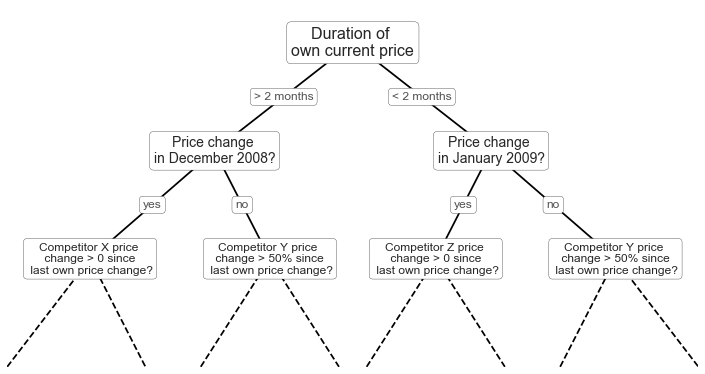
\includegraphics[scale=.65]{rf_tree.png}
    \label{Figure 1}
\end{figure}
\begin{figure}[b]
    \centering
        \caption{Nearest Neighbor Data Clustering Example}
    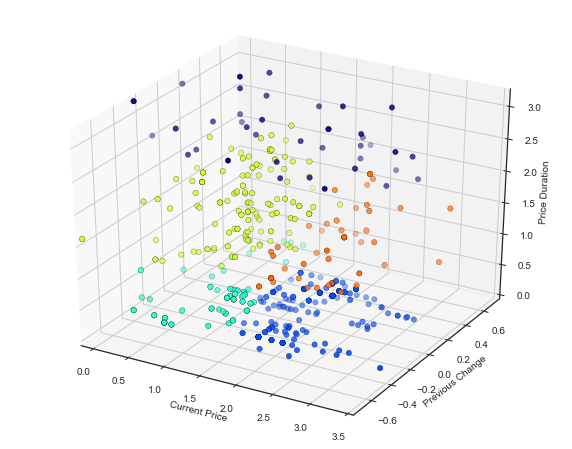
\includegraphics[scale=.75]{kmeans_cluster2.png}
    \label{Figure 2}
\end{figure}

\begin{figure}[b]
    \centering
        \caption{Out of Sample RMSE vs. Regulation Size (Ridge Regression)}
    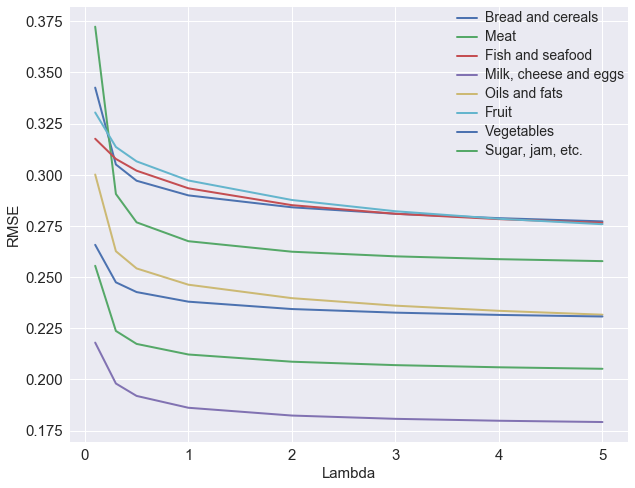
\includegraphics[scale=.65]{lambda.png}
    \label{Figure 3}
\end{figure}


\begin{figure}[ht]
  \caption{Receiver Operating Characteristic Curves - Price Increase vs. Decrease}
  \begin{subfigure}[b]{0.5\textwidth}
    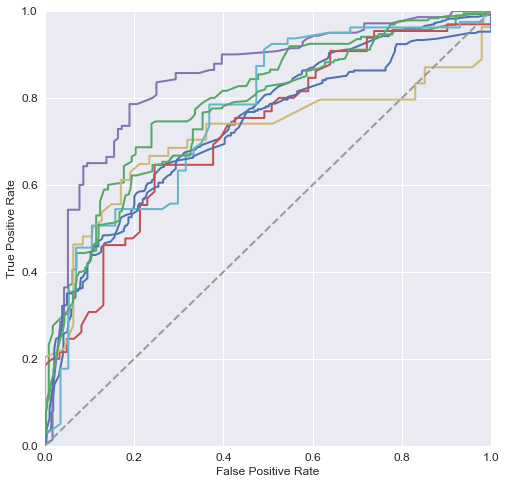
\includegraphics[width=\textwidth]{logistic_roc.png}
    \caption{Logistic}
  \end{subfigure}
  %
  \begin{subfigure}[b]{0.5\textwidth}
    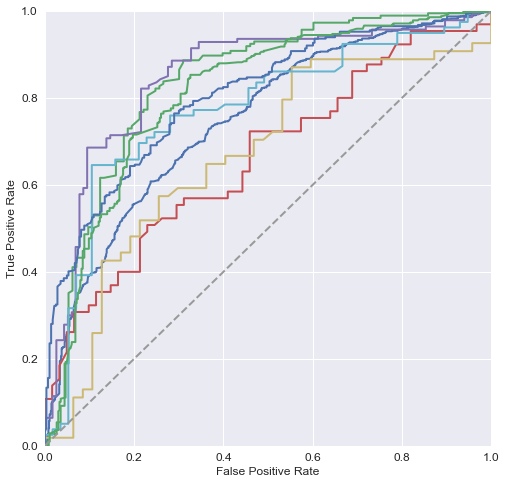
\includegraphics[width=\textwidth]{ridge_roc.png}
    \caption{Ridge}
  \end{subfigure}
   \begin{subfigure}[d]{0.5\textwidth}
    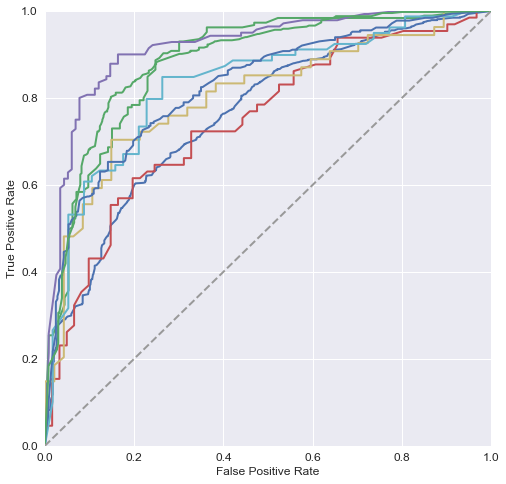
\includegraphics[width=\textwidth]{random_forest_roc.png}
    \caption{Random Forest}
  \end{subfigure}
  %
  \begin{subfigure}[d]{0.5\textwidth}
    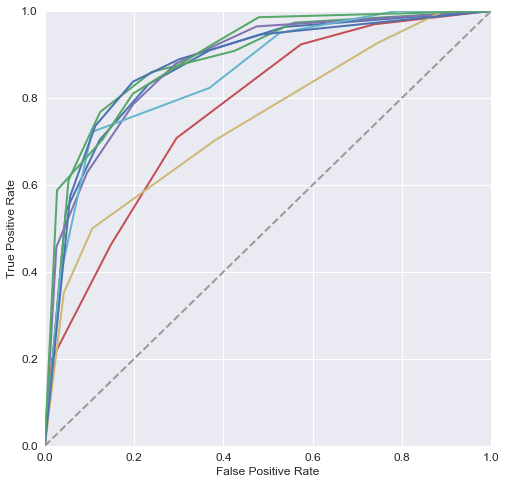
\includegraphics[width=\textwidth]{knn_roc.png}
    \caption{KNN}
  \end{subfigure}
  ROC curves for estimating the direction of price change for eight product categories: Breads and cereals, meat, fish and seafood, milk, cheese and eggs, oils and fats, fruit, vegetables, and sugar/jam/honey/chocolate. Dotted 90 degree line specifies luck (i.e., accuracy of algorithm is equivalent to coin flip).
  \label{Figure 2}
\end{figure}


\begin{figure}[ht]
    \centering
    \caption{KNN Reset Price Trajectory (Grocery)}
    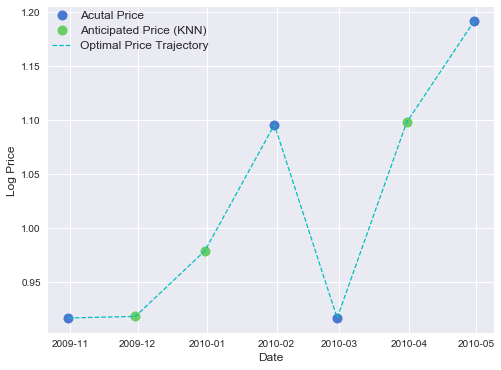
\includegraphics[scale=.8]{knn_reset.png}
    \label{Figure 3}
\end{figure}

\begin{figure}[ht]
    \centering
       \caption{Linear Regression Reset Price Trajectory (Grocery)}
    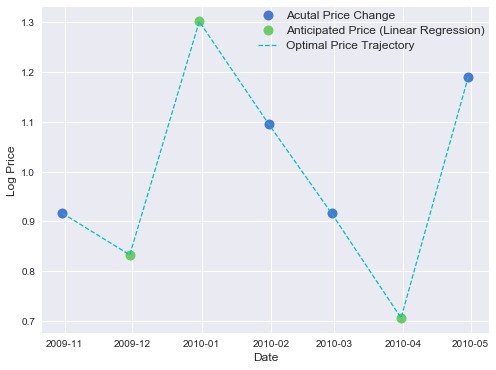
\includegraphics[scale=.8]{linear_reset.png}
    \label{Figure 4}
\end{figure}

\begin{figure}[ht]
    \centering
    \caption{KNN Reset Price Trajectory (Household Appliances)}
    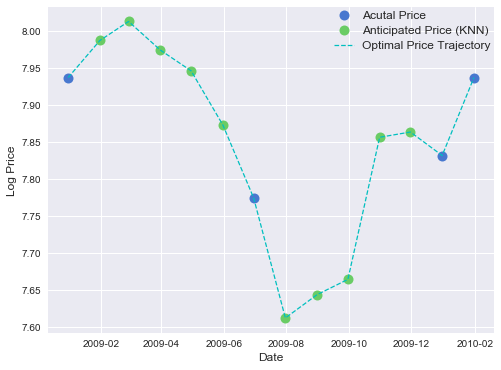
\includegraphics[scale=.8]{knn_reset2.png}

\end{figure}

\begin{figure}[ht]
    \centering
       \caption{Linear Regression Reset Price Trajectory (Household Appliances)}
    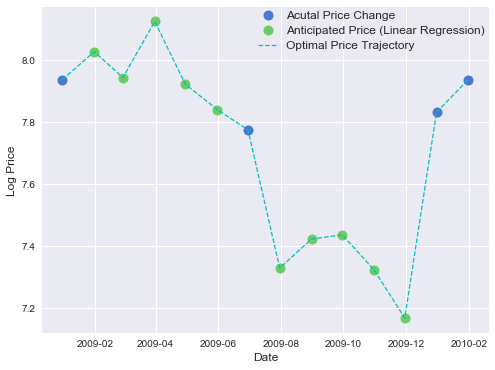
\includegraphics[scale=.8]{linear_reset2.png}

\end{figure}

\end{document}
